\subsection{Heat expansion}
%Divide into subsections if needed. 
The expression that describes thermal expansion for a volume in solids is
\begin{equation}
	\alpha_v=\frac{1}{V}\frac{dV}{dT}
	\label{eq2}
\end{equation} 
where $\alpha_v$ is the thermal expansion coefficient of the volume, $V$ is the volume of the solid and $T$ is the temperature of the solid.
As the solid in this case is a long metallic rod eq. \eqref{eq2} can be approximated as

\begin{equation}
	\alpha_L=\frac{1}{L}\frac{dL}{dT}
	\label{eq3}
\end{equation}

where $\alpha_L$ is the thermal expansion coefficient of the length $L$ of the rod. Eq. \eqref{eq3} can then be approximated to
\begin{equation}
	\alpha_L=\frac{1}{L}\frac{\Delta L}{\Delta T}
	\label{eq4}
\end{equation}
where $\Delta L$ and $\Delta T$ is the change in the length and temperature of the rod.

\subsection{Michelson interferometer}
%Divide into subsections if needed.
The working principle behind the Michelson interferometer is that a beam of light is split so that the resulting beams can be led through two optical paths of different lengths and later be recombined to an interference pattern.
 
\begin{figure}[htb]
	\centering
	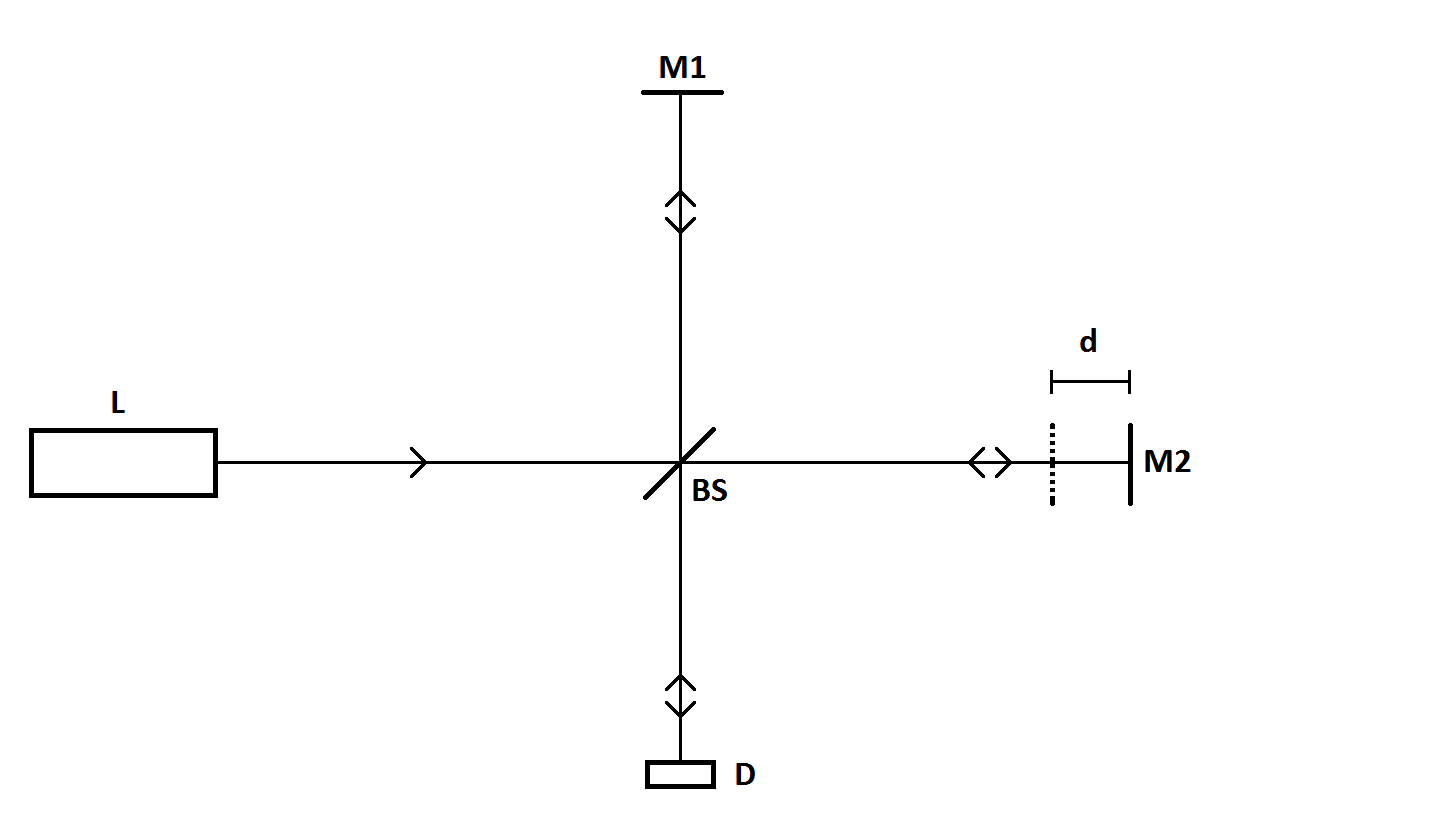
\includegraphics[scale=0.25]{img/Int1}
	\caption{Schematic illustration of an Michelson interferometer. In the figure $L$ is the light source, $BS$ is the beam-splitter, $M1$ and $M2$ are the two mirrors, $D$ is the detector and $d$ is the displacement of $M2$}
	\label{fig1}
\end{figure}

In fig. \ref{fig1} the light emanating from the light source gets split up at a beam-splitter creating two beams. We will call these two beams $B1$ (the one travelling upwards in fig. \ref{fig1}) and $B2$ (the one travelling to the right).
The beam $B1$ gets reflected in the beam-splitter and directed towards a mirror $M1$, travelling some distance $l_1$ to a mirror. It is then reflected back towards the beam-splitter, where it passes through and hit the detector after travelling a distance $l_d$.\\

For the other beam, $B2$, we see that it passes through the beam splitter and travels some distance $l_2$, gets reflected back to the beam splitter and is directed to the detector.\\

When we consider the phase shift between these beams as they go through the system; both beams gets reflected the same number of times. This means that the optical path length difference---and therefore also the phase shift between the beams---will only depend on the actual travelling distances $l_1$ and $l_2$ (the travelling distances shared by both beams will not contribute to the optical path difference and are therefore not of interest).
From this we can see that the optical path difference of the beams can be expressed as
\begin{equation}
	\Delta l=2l_1-2l_2=2(l_1-l_2)
	\label{eq5}
\end{equation}
where $\Delta l$ is the optical path difference.
For this phase shift to result in constructive interference the optical path difference must be an integer multiple of the wavelength. This condition and eq. \ref{eq5} gives us the following expression
\begin{equation}
	m\lambda=\Delta l=2(l_1-l_2), \qquad m=0,1,2,...
	\label{eq6}
\end{equation}
where $\lambda$ is the wavelength of the light and $m$ is an integer numbering the interference fringes.\\

In our application of this interferometer the length $l_2$ is not going to be fixed but it will shift with some displacement, $d$, that is dependent on time. If this is inserted into eq. \ref{eq6} we get
\begin{equation}
	m\lambda=\Delta l=2(l_1-l_2+d).
	\label{eq7}
\end{equation}
From this we see that as this displacement changes, the value of $m$ will change. This will result in a movement of the interference fringes which can be detected and used to measure the displacement.